\subsection{UC19: Checkout}
        \label{sec:UC19}
            \begin{figure}[!ht]
                \caption{Diagramma di UC19: Checkout}
                \vspace{10px}
                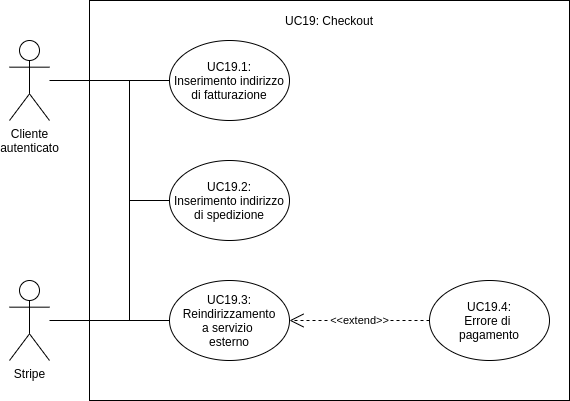
\includegraphics[scale=0.5]{../../../Images/AnalisiRequisiti/UC19}
                \centering
            \end{figure}
                \begin{itemize}
                \item \textbf{Descrizione:} caso d'uso per la creazione di un nuovo ordine e l'acquisto dei prodotti inseriti nel carrello;
                \item \textbf{Attore Primario:} cliente autenticato;
                \item \textbf{Attore Secondario:} Stripe, gestore di pagamenti di terze parti;
                \item \textbf{Precondizione:} il cliente si trova sul carrello e ha già inserito almeno un prodotto;
                \item \textbf{Input:} il cliente clicca il bottone per iniziare il checkout;
                \item \textbf{Postcondizione:} l'ordine viene emesso e aggiunto alla lista degli ordini di quel cliente; i prodotti acquistati vengono rimossi dal carrello e viene diminuita la quantità dal deposito del venditore;
                \item \textbf{Scenario Principale:} 
                    \begin{itemize}
                        \item il cliente preme sul pulsante per entrare nella sezione del checkout;
                        \item il cliente inserisce i dati di fatturazione (\hyperref[sec:UC19.1]{\underline{UC19.1}}) e, se diversi, i dati di spedizione (\hyperref[sec:UC19.2]{\underline{UC19.2}});
                        \item vengono inseriti eventuali costi di spedizione;
                        \item il cliente viene reindirizzato al servizio di pagamento esterno, dove inserisce i dati di pagamento;
                        \item l'ordine è emesso e segnato come completato.
                    \end{itemize}
                \item \textbf{Estensioni:}
                    \begin{itemize}
                        \item se il cliente decide di non completare il checkout, può uscire dalla pagina senza causare modifiche al carrello;
                        \item se il pagamento ha avuto esito negativo, l'ordine non viene emesso e quindi è necessario ricominciare il pagamento.
                    \end{itemize}
            \end{itemize}
            \subsubsection{UC19.1: Inserimento dell'indirizzo di fatturazione}
            \label{sec:UC19.1}
                \begin{itemize}
                    \item \textbf{Descrizione:} Sezione per l'inserimento dell'indirizzo fatturazione;
                    \item \textbf{Attore Primario:} cliente autenticato;
                    \item \textbf{Precondizione:} il cliente si trova nella fase di checkout;
                    \item \textbf{Input:} il cliente inserisce i dati richiesti dalla pagina;
                    \item \textbf{Postcondizione:} si procede con la fase successiva del checkout (\hyperref[sec:UC19.2]{\underline{UC19.2}})
                    \item \textbf{Scenario Principale:} il cliente inserisce negli appositi spazi i dati per completare l'indirizzo di fatturazione.
                \end{itemize}
            \subsubsection{UC19.2: Inserimento dell'indirizzo di spedizione}
            \label{sec:UC19.2}
                \begin{itemize}
                    \item \textbf{Descrizione:} Sezione per l'inserimento dell'indirizzo spedizione;
                    \item \textbf{Attore Primario:} cliente autenticato;
                    \item \textbf{Precondizione:} il cliente si trova nella fase di checkout;
                    \item \textbf{Input:} il cliente inserisce i dati richiesti dalla pagina, oppure clicca un pulsante se l'indirizzo di spedizione è lo stesso di quello di fatturazione;
                    \item \textbf{Postcondizione:} si procede con la fase successiva del checkout (\hyperref[sec:UC19.3]{\underline{UC19.3}})
                    \item \textbf{Scenario Principale:} il cliente inserisce negli appositi spazi i dati per completare l'indirizzo di spedizione oppure clicca il pulsante per autocompletarli se è il medesimo di quello di fatturazione.
                \end{itemize}
            \subsubsection{UC19.3: Reindirizzamento al servizio di pagamento esterno}
            \label{sec:UC19.3}
                \begin{itemize}
                    \item \textbf{Descrizione:} Sezione per il pagamento dell'ordine da effettuare;
                    \item \textbf{Attore Primario:} cliente autenticato;
                    \item \textbf{Attore Secondario:} Stripe, gestore di pagamenti di terze parti;
                    \item \textbf{Precondizione:} il cliente ha inserito i dati per la fatturazione e la spedizione nella sezione del checkout;
                    \item \textbf{Input:} il cliente preme il pulsante per il pagamento;
                    \item \textbf{Postcondizione:} il pagamento ha avuto esito positivo, l'ordine viene confermato e viene decrementata la quantità dei prodotti disponibili al venditore, in base al numero di prodotti acquistati dal cliente;
                    \item \textbf{Scenario Principale:}
                    \begin{itemize}
                        \item il cliente preme sul pulsante e viene reindirizzato al servizio esterno per eseguire il pagamento;
                        \item il cliente inserisce i propri dati ed esegue il pagamento;
                        \item il pagamento è riuscito e l'ordine viene confermato.
                    \end{itemize}
                    \item \textbf{Estensioni:}
                    \begin{itemize}
                        \item il pagamento non è riuscito, viene visualizzato un errore di pagamento (\hyperref[sec:UC19.4]{\underline{UC19.4}}) e si viene reindirizzati alla pagina del checkout per riprovare.
                    \end{itemize}
                \end{itemize}
            \subsubsection{UC19.4: Errore di pagamento}
            \label{sec:UC19.4}
                \begin{itemize}
                    \item \textbf{Descrizione:} visualizzazione di un errore per un fallimento nella fase di pagamento;
                    \item \textbf{Attore Primario:} Stripe
                    \item \textbf{Precondizione:} il cliente ha inserito i dati del pagamento;
                    \item \textbf{Input:} Stripe ritorna un errore nel risultato del pagamento;
                    \item \textbf{Postcondizione:} viene visualizzato un messaggio di errore, successivamente il cliente viene reindirizzato alla sezione del checkout;
                \end{itemize}